\documentclass{standalone}
\usepackage{tikz}
\usepackage{ctex,siunitx}
\setCJKmainfont{Noto Serif CJK SC}
\usepackage{tkz-euclide}
\usepackage{amsmath}
\usetikzlibrary{patterns, calc}
\usetikzlibrary {decorations.pathmorphing, decorations.pathreplacing, decorations.shapes,}

\begin{document}
\small
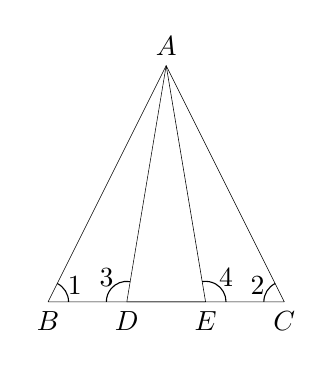
\begin{tikzpicture}[>=stealth,scale=1.0]
  \tkzSetUpPoint[fill=black]
  % \useasboundingbox(-1,-0.75)rectangle(3.7,1.4);
  \tkzDefPoints{0/3/A, -1.5/0/B, 1.5/0/C, -.5/0/D, .5/0/E}
  \tkzDrawPolygon(A,B,C)
  \tkzDrawPolygon(A,D,E)
  \tkzLabelPoints[below](B,C,D,E)
  \tkzLabelPoints[above](A)
  \tkzMarkAngles[mark=none, size=.26](C,B,A A,C,B A,D,B C,E,A)
  \tkzLabelAngle[pos=.4](C,B,A){1}
  \tkzLabelAngle[pos=.4](A,C,B){2}
  \tkzLabelAngle[pos=.4](A,D,B){3}
  \tkzLabelAngle[pos=.4](C,E,A){4}
\end{tikzpicture}
\end{document}